\documentclass[11pt]{article}
\usepackage[margin=1in]{geometry}
\usepackage[T1]{fontenc}
\usepackage{mathptmx}
\usepackage{courier}
\usepackage{microtype}
\usepackage{amsmath,amssymb}
\usepackage{graphicx}
\usepackage{booktabs}
\usepackage{multirow}
\usepackage[numbers,sort&compress]{natbib}
\usepackage{xcolor}
\usepackage[colorlinks=true,linkcolor=blue!60!black,citecolor=blue!60!black,urlcolor=blue!60!black]{hyperref}
\usepackage{caption}
\captionsetup{font=small,labelfont=bf}

\newcommand{\lr}{\ensuremath{\leftrightarrow}}

\title{Separately Trained Senses Converge on Shared Latent Structure:\\
An Empirical Check of Identifiability Predictions\\ Without Shared Data}

\author{Jonathan Bussing\\
Independent Researcher\\
\texttt{jbussing@ucsd.edu}}

\date{Preprint, version 1.0.1 \,$\cdot$\, October 2026\\[2pt] \small\href{https://doi.org/10.5281/zenodo.23445191}{doi:10.5281/zenodo.23445191} \,$\cdot$\, \url{https://github.com/jbussin/senses-converge}}

\begin{document}
\maketitle

\begin{abstract}
Identifiability theory for contrastive learning predicts that an encoder trained with suitable positive pairs recovers the latent structure behind its inputs, so separately trained networks that perceive a common world should converge on its shared structure without shared training data. This is one proposed explanation for the Platonic Representation Hypothesis, whose evidence comes mostly from models trained on overlapping human-generated data. We check the prediction in a small synthetic world: an ``eye'' (rendered images) and an ``ear'' (rendered sounds) each perceive eight latent properties of every object, a controlled number of them shared, and each network is trained alone, without labels, on its own objects. Over three seeds, with permutation-calibrated mutual nearest-neighbor alignment, the learners stay at the null level when they share nothing and converge monotonically as the shared fraction grows; from half overlap upward, each learner's features also move toward the true shared properties. Among four learning rules, strong convergence occurred only with the one that approximates the theory's assumptions, contrastive learning between glimpses of an object that drifts between them, and peaked at an intermediate drift; the sound learner, which does not improve at all without drift, discriminates the rules most clearly. With the present learners, the convergence is too weak for unpaired Gromov--Wasserstein matching to recover which image goes with which sound. Partially shared perception also makes fine-grained alignment fall as evaluation sets grow while coarse alignment holds, as recently reported for language and vision models, suggesting a way to reconcile that finding with convergence on shared structure. A calibrated check with Pythia and DINOv2 reproduces the reported language--vision size trend at small scale. The study is confirmatory and small: it shows that a shared world can produce convergence without shared data, and makes no claim about how much of the convergence between web-trained models this explains.
\end{abstract}

%======================================================================
\section{Introduction}

The Platonic Representation Hypothesis \citep{huh2024platonic} proposes that neural networks trained separately---on different data, with different architectures and objectives, even in different modalities---are converging toward a shared representation of the world, and that convergence strengthens with capability. Evidence came largely from mutual nearest-neighbor alignment between language and vision models on about a thousand image--caption pairs.

The hypothesis is now actively debated. \citet{koepke2026cave} find that cross-modal alignment degrades substantially when the evaluation set grows from about a thousand to millions of samples, that the one-caption-per-image setting inflates it, and that newer language models do not continue the reported trend. \citet{groger2026aristotelian} show that common similarity metrics are confounded by network width and depth---in particular, taking the maximum over layer pairs inflates scores for deeper models---and propose permutation-based calibration; after calibration, global convergence largely disappears while local neighborhood agreement persists. \citet{you2026structure} similarly find that relational structure converges more robustly than metric geometry.

A separate and more basic question is \emph{why} any convergence occurs. For models trained on internet data, a natural explanation is that they share data: overlapping corpora and captioned images carry the same human categories and emphases. A competing explanation is that they share a world, and any learner that captures the world's regularities is pushed toward the same structure. On web-scale data the two explanations make the same prediction.

This paper checks the shared-world explanation in a setting where the two come apart. We construct a synthetic world whose objects are perceived by two senses---an ``eye'' that sees rendered images and an ``ear'' that hears rendered sounds. The senses share a controllable number of the objects' latent properties. Each sense's network is trained alone, without labels, on its own stream of objects; the two networks never share a training example. Because the world is constructed, we can measure not only whether the two networks converge on each other but whether each converges on the world's true latent structure. The working hypothesis is:

\begin{quote}
\textbf{(H)} Learners that capture the world's regularities converge on the part of the world they both perceive, and the structure they converge on belongs to the world rather than to the learners.
\end{quote}

\paragraph{Scope.} This is a confirmatory study. Under existing identifiability theory for contrastive learning \citep{zimmermann2021contrastive,vonkugelgen2021self,daunhawer2023identifiability}, convergence in our main setting is the expected outcome, and the world was designed so that the theory's assumptions can hold. What the theory does not directly cover is finite networks trained briefly on rendered perceptual inputs, with no paired or shared training data; the experiment checks that its prediction survives in that regime. We make no claim about how much of the convergence between web-trained models the mechanism explains.

\paragraph{Contributions.}
\begin{itemize}
  \item A multi-seed, permutation-calibrated check, in a synthetic world with two senses, disjoint self-supervised training, and ground-truth latents, that separately trained networks converge on the structure they share, and that this requires the learning rule that meets the theory's assumptions (Section~\ref{sec:synthetic}).
  \item A drift sweep: convergence peaks at an intermediate drift, and choosing the drift matters more than tripling training time (Section~\ref{sec:drift}).
  \item A negative result: despite significant convergence, unpaired matching cannot recover which image goes with which sound (Section~\ref{sec:unpaired}).
  \item A candidate mechanism for the reported fall of cross-modal alignment with evaluation-set size \citep{koepke2026cave}: partially shared perception erodes fine-grained agreement as sampling becomes denser while coarse agreement holds, for perfect and trained learners alike (Sections~\ref{sec:scale} and~\ref{sec:disc}).
  \item A calibrated language--vision sanity check in the original evaluation regime (Section~\ref{sec:textvision}), and a note on degenerate layers that inflate layer-maximized scores (Section~\ref{sec:metric}).
\end{itemize}

%======================================================================
\section{Related work}

\paragraph{Representational convergence and its critics.} Beyond \citet{huh2024platonic}, related evidence includes unsupervised alignment of word embeddings across languages \citep{conneau2018word}, zero-shot communication through relative representations \citep{moschella2023relative}, and translation between text-embedding spaces without paired data \citep{jha2025vec2vec}. The critiques of \citet{koepke2026cave}, \citet{groger2026aristotelian}, and \citet{you2026structure} discussed above shape our choices: we use a local neighborhood metric, calibrate it against a permutation null that repeats the full layer search, and do not draw conclusions about evaluation scale from a 1{,}024-item evaluation.

\paragraph{Synthetic studies of convergence.} \citet{tjandrasuwita2025emergence} construct two synthetic modalities that share redundant features and carry unique ones, train unimodal encoders on a common supervised label, and measure CKA; they find that alignment emerges and grows with capacity only when redundancy is high. Our overlap manipulation is closely related. The differences are that our networks are trained without labels, on disjoint objects, from rendered images and sounds rather than feature vectors, and that we measure alignment with the ground-truth latent in addition to cross-model alignment. \citet{park2026convergent} studies how tasks defined over a single synthetic world shape representation geometry, including divergent tasks that harm integration. \citet{li2026worldmodels} find convergence among world models with different visual encoders trained on identical transition data in simulated environments; our design removes shared training data.

\paragraph{Identifiability of self-supervised learning.} Contrastive learning with positive pairs drawn from a local conditional around each latent inverts the generative process up to a simple transformation under suitable assumptions \citep{zimmermann2021contrastive}; augmentation-based self-supervision isolates the invariant content block \citep{vonkugelgen2021self}; and multimodal contrastive learning identifies the latent factors shared across modalities \citep{daunhawer2023identifiability}. Empirically, the choice of views matters, with a sweet spot in how much information they share \citep{tian2020views}. Slow feature analysis \citep{wiskott2002slow} expresses a related intuition: the causes of sensation change more slowly than sensation. Reconstruction objectives carry no comparable guarantee.

\paragraph{Brains, species, and perception.} Representational similarity analysis compares similarity structure across brains and models \citep{kriegeskorte2008rsa}; human and macaque inferior temporal cortex share categorical structure \citep{kriegeskorte2008matching}, and task-optimized networks predict ventral-stream responses \citep{yamins2016goal}. Whether minds with different senses can share a conceptual map is an old question \citep{nagel1974bat}, and modeling animal communication directly from audio makes it empirical \citep{andreas2022whales}. Our overlap manipulation is a toy version of partially shared perception.

%======================================================================
\section{Measuring alignment}
\label{sec:metric}

For $N$ items with features $A=\{a_i\}$ and $B=\{b_i\}$, let $\mathcal{N}^A_k(i)$ be the $k$ nearest neighbors of item $i$ under cosine similarity in $A$, excluding $i$. Mutual $k$-NN alignment \citep{huh2024platonic} is
\begin{equation}
  m_k(A,B) \;=\; \frac{1}{N}\sum_{i=1}^{N} \frac{\lvert \mathcal{N}^A_k(i)\,\cap\,\mathcal{N}^B_k(i)\rvert}{k}.
\end{equation}
Chance is $k/(N-1)\approx 0.010$ for $k=10$, $N=1024$. Following \citet{huh2024platonic}, we compute $m_k$ for every pair of layers and take the maximum, $M(A,B)=\max_{\ell,\ell'} m_k(A_\ell,B_{\ell'})$.

\paragraph{Permutation calibration.} Maximizing over layer pairs inflates scores, more so for deeper networks \citep{groger2026aristotelian}. We therefore compare each score with a null distribution obtained by permuting the rows of $B$ and \emph{repeating the full layer search}, $M(A,\pi B)$, for 20 random permutations $\pi$. We report the null mean $\mu_0$, the calibrated score $\tilde M = (M-\mu_0)/(1-\mu_0)$, which is zero at the null level and one for identical neighborhoods, and the permutation $p$-value $(1+\#\{M(A,\pi B)\geq M\})/21$, whose minimum is $0.048$. This follows the spirit of \citet{groger2026aristotelian}; it is not their exact estimator.

\paragraph{Uncertainty.} In the synthetic experiments we train each configuration with three seeds; a seed changes the world's renderers, the networks' initial weights, the training streams, and the test objects, and we report mean $\pm$ standard deviation across seeds. In the text--vision check, where models are fixed, we report the standard deviation of the score at the selected layer pair over 30 random 80\% subsets of items, which understates sampling variability.

\paragraph{A pitfall: degenerate layers.} In an early version of our pipeline, a shuffled control scored two to three times chance. The cause was the Vision Transformer's input layer, whose CLS token is identical for every image: all similarities tie, every row gets the same arbitrary neighbors, and these overlap with the other representation's hub items \citep{radovanovic2010hubs} regardless of pairing. We exclude layers whose features have near-zero spread across items (mean distance to the centroid below $10^{-4}$ of the mean norm).

%======================================================================
\section{A synthetic world with two senses}
\label{sec:synthetic}

\subsection{Design}

\paragraph{The world.} Each object has latent properties drawn uniformly from $[0,1]$. Each sense perceives $D=8$ of them, of which $S\in\{0,2,4,6,8\}$ are shared with the other sense and $D-S$ are private. Each sense renders its latent vector through a fixed, randomly initialized two-layer network, so no learner has access to latent coordinates. The \emph{eye} sees six colored Gaussian blobs on a $32\times32$ RGB canvas; the \emph{ear} hears 1{,}024 samples of six decaying tones. Every glimpse adds nuisance (shift, brightness, and noise for the eye; onset delay, phase, volume, and noise for the ear). Section~\ref{sec:formal} gives the formal model and Appendix~\ref{app:render} the renderers.

\paragraph{The learners.} Each learner is a three-layer strided convolutional encoder with base width $w$ (channels $w,2w,4w$) and a 32-dimensional embedding; the ear first applies a fixed log-magnitude spectrogram (a ``cochlea''). Training uses Adam (learning rate $10^{-3}$), batch 256, and 8{,}000 steps. \textbf{The two learners never share a training object, never see the other modality, and never see a cross-modal pair.}

\paragraph{Learning rules.} Four rules, fixed before the runs reported here: \texttt{recon}, denoising reconstruction on fresh objects; \texttt{contrast\_fixed}, InfoNCE \citep{chen2020simclr} between two glimpses of the same object from a fixed set of 6{,}000 objects; \texttt{contrast\_fresh}, the same with fresh objects every step; and \texttt{contrast\_drift}, the same with the object drifting between glimpses by Gaussian noise of scale $\sigma$ ($0.05$ unless stated). \texttt{recon} differs from \texttt{contrast\_fresh} only in its objective, and each contrastive rule differs from the next in one respect. Only \texttt{contrast\_drift} approximates the assumptions of \citet{zimmermann2021contrastive}, so theory predicts that only it recovers the latent geometry; the others serve as contrasts.

\paragraph{Evaluation.} After training, both learners perceive the same 1{,}024 held-out objects, one glimpse per sense. We measure eye\lr{}ear alignment $M$ (maximized over the three convolutional outputs and the embedding, with its calibration), the same at initialization, and \emph{eye\lr{}truth} and \emph{ear\lr{}truth}: $M$ between each learner's features and the true shared properties, which exist only because the world is constructed. Raw inputs do not align (raw pixels versus raw waveforms: $m_k=0.010$ at $S=4$, $0.012$ at $S=8$).

\paragraph{Experiments.} (A) overlap sweep, $S\in\{0,2,4,6,8\}$, $w=32$, \texttt{contrast\_drift}; (B) learning rules, $S=8$, $w=32$; (C) width sweep, $S=4$, $w\in\{4,16,32,64\}$; and, as a follow-up, (D) a drift sweep and (E) longer training, both at $S=8$, $w=32$ (Section~\ref{sec:drift}); (F) an unpaired matching test on retrained drift-sweep configurations (Section~\ref{sec:unpaired}); and (G) an evaluation-size test (Section~\ref{sec:scale}). Each configuration uses seeds 0, 1, 2.

\subsection{Formal setup and predictions}
\label{sec:formal}

\paragraph{Generative model.} Fix $D=8$ and $S\in\{0,\dots,D\}$. For each object,
\begin{equation}
  s\sim\mathcal U([0,1]^S),\qquad p^{e},\,p^{a}\sim\mathcal U([0,1]^{D-S}),\qquad
  z^{e}=(s,p^{e}),\quad z^{a}=(s,p^{a})\in[0,1]^D,
  \label{eq:latents}
\end{equation}
with $s$, $p^{e}$, $p^{a}$ independent. Every glimpse draws nuisance $\nu$ independently of the latents, and the senses produce
\begin{equation}
  x^{e}=R_{e}\big(\phi_{e}(z^{e}),\nu^{e}\big),\qquad x^{a}=R_{a}\big(\phi_{a}(z^{a}),\nu^{a}\big),
  \qquad \phi_m(z)=\sigma\!\big(W^m_2\tanh(W^m_1(2z-\mathbf 1)+b^m)\big),
  \label{eq:render}
\end{equation}
where $\sigma$ is the logistic function and the weights are fixed Gaussian draws. We write $g_m(z,\nu)=R_m(\phi_m(z),\nu)$ for the full rendering map of sense $m$. The eye's six blobs take their positions, widths, and colors from $\phi_e$; the ear's six tones take their frequencies, amplitudes, and decay rates from $\phi_a$ (Appendix~\ref{app:render}).

\paragraph{Learners and objectives.} Each sense $m\in\{e,a\}$ has an encoder $f_m$ with values in $\mathbb R^{32}$ (the ear's encoder first applies the fixed map $C(x)=\log(1+10\,\lvert\mathrm{STFT}(x)\rvert)$) and, for the contrastive rules, a projection head $h_m$. For a batch of $B$ positive pairs, let $\{y_a\}_{a=1}^{2B}$ be the $2B$ glimpses, $a^+$ the partner of $a$, and $u_a=h_m(f_m(y_a))$. The InfoNCE loss is
\begin{equation}
  \mathcal L_{\mathrm{NCE}}=-\frac{1}{2B}\sum_{a=1}^{2B}\log\frac{\exp\big(\cos(u_a,u_{a^+})/\tau\big)}{\sum_{b\neq a}\exp\big(\cos(u_a,u_b)/\tau\big)},\qquad \tau=0.2 .
\end{equation}
The contrastive rules differ only in how a positive pair $(z,z')$ is drawn; its two glimpses are $g_m(z,\nu)$ and $g_m(z',\nu')$ with independent nuisance:
\begin{align}
  \texttt{contrast\_fixed}:&\quad z\sim\mathcal U(\mathcal Z_{\mathrm{fix}}),\ \lvert\mathcal Z_{\mathrm{fix}}\rvert=6000,\quad z'=z;\\
  \texttt{contrast\_fresh}:&\quad z\sim\mathcal U([0,1]^D),\quad z'=z;\\
  \texttt{contrast\_drift}:&\quad z\sim\mathcal U([0,1]^D),\quad z'=\mathrm{clip}_{[0,1]}(z+\sigma\varepsilon),\ \varepsilon\sim\mathcal N(0,I_D),\ \sigma=0.05\ \text{unless stated}.
  \label{eq:drift}
\end{align}
The reconstruction rule uses a decoder $d_m$ and $\mathcal L_{\mathrm{rec}}=\mathbb E\,\lVert d_m(f_m(x+\eta))-T_m(x)\rVert^2$ with $\eta\sim\mathcal N(0,0.1^2 I)$, $T_e=\mathrm{id}$, and $T_a=C$. The eye and the ear draw $z$ from independent streams, so no latent vector is shared between their training sets.

\paragraph{Quantities reported.} For $N$ test objects, let $F^m_\ell\in\mathbb R^{N\times d_\ell}$ be sense $m$'s features at layer $\ell$, $Z^{e},Z^{a}\in[0,1]^{N\times D}$ the true latent matrices, and $Z^{\mathrm{sh}}\in[0,1]^{N\times S}$ the shared coordinates. We report $M(F^e,F^a)$ (eye\lr{}ear), $M(F^m,Z^{\mathrm{sh}})$ (eye\lr{}truth, ear\lr{}truth), and two reference levels obtained by applying the same metric to the latents themselves: $M(Z^e,Z^a)$ and $M(Z^m,Z^{\mathrm{sh}})$. These are the scores of a learner whose features have exactly the neighborhood structure of its latent vector. Averaged over our three test sets, $M(Z^e,Z^a)=0.010,\,0.030,\,0.082,\,0.259,\,1.000$ for $S=0,2,4,6,8$, and $M(Z^m,Z^{\mathrm{sh}})=0.028,\,0.13,\,0.37,\,1.000$ for $S=2,4,6,8$ (eye and ear values agree to within 0.004). Both are below 1 whenever private properties exist, because the private coordinates reshuffle neighborhoods. Like all neighborhoods in this paper, those of the latent vectors use cosine similarity, here on the latents as generated in $[0,1]$; this ignores their norm and, for $S=2$, reduces the shared coordinates to a single angle, whereas drift and the theory are Euclidean. The truth columns and reference levels therefore measure agreement with this view of the latents. The truth scores use a 5-permutation null.

\paragraph{Predictions.}
\begin{itemize}
  \item[\textbf{P0}] \emph{No shared properties.} If $S=0$, the eye's and ear's test inputs are independent, and so are their trained networks, which were trained on independent streams. Conditional on the eye's features, the ear's features are then i.i.d.\ across objects and independent of them, so the ear's neighbor set of each object is a uniformly random $k$-subset of the other $N-1$ objects (ties have probability zero). Hence $\mathbb E\,m_k(F^e_\ell,F^a_{\ell'})=k/(N-1)$ for every layer pair, and the layer-maximized score $M$ has the same distribution as the permutation null: the calibrated score is zero in expectation.
  \item[\textbf{P1}] \emph{Drift.} \citet{zimmermann2021contrastive} show that when latents have a uniform marginal on a convex set, positive pairs come from a conditional concentrated around each latent according to a distance, the generator is injective, and the encoder minimizes the contrastive loss, the encoder recovers the latents up to a simple transformation, such as an affine map. \texttt{contrast\_drift} approximates these conditions: a uniform marginal on the convex set $[0,1]^D$ and a local Gaussian conditional, exact away from the boundary. The theory's other assumptions are not guaranteed here: injectivity of $g_m$ in the presence of nuisance, the exact form of the conditional near the boundary, cosine rather than distance-based similarity, and infinite capacity and data. The prediction is therefore qualitative: under drift, $M(F^m,Z^{\mathrm{sh}})$ and $M(F^e,F^a)$ should rise with training toward their reference levels, and should increase with $S$.
  \item[\textbf{P2}] \emph{No drift.} In \texttt{contrast\_fixed} and \texttt{contrast\_fresh}, the two glimpses share $z$ exactly and differ only in nuisance. \citet{vonkugelgen2021self} show that such objectives identify the invariant block---here all of $z$---only up to an invertible map, which need not preserve distances or neighborhoods. A learner can then encode the latents while distorting their local geometry, so these rules carry no prediction that neighborhood alignment approaches the reference levels.
  \item[\textbf{P3}] \emph{Reconstruction.} $\mathcal L_{\mathrm{rec}}$ rewards retaining whatever is needed to reconstruct $x$, including nuisance, and carries no identifiability guarantee.
\end{itemize}
Figure~\ref{fig:synth} and Table~\ref{tab:synth} test P0--P3.

\subsection{Results}

\begin{figure}[t]
  \centering
  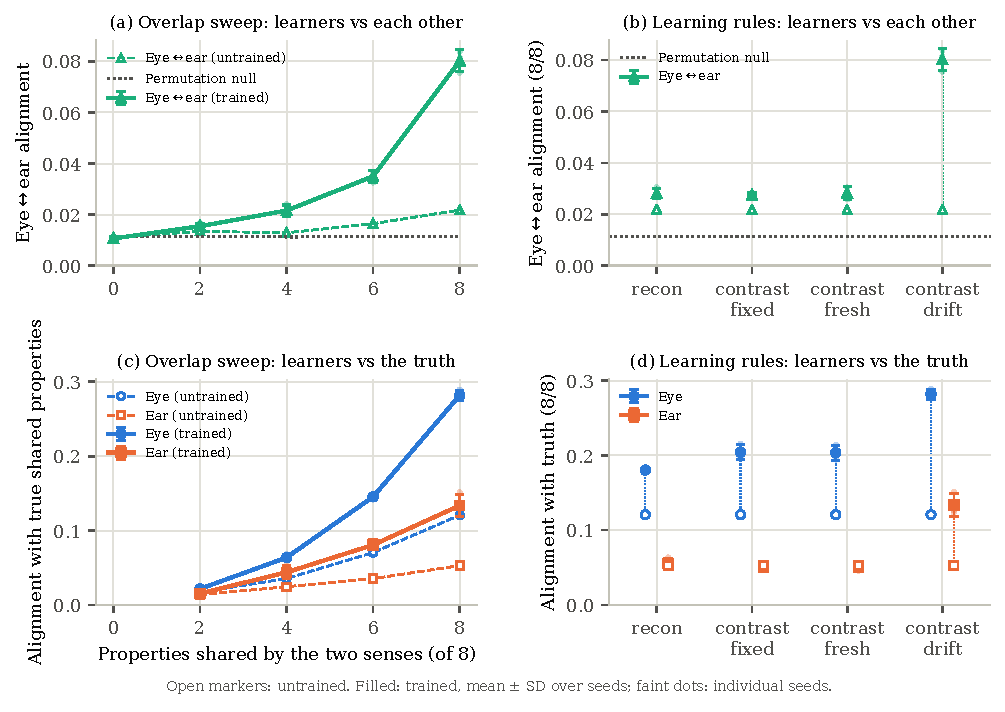
\includegraphics[width=\linewidth]{figures/fig_synth_overlap_rules.pdf}
  \caption{Synthetic world, three seeds per configuration. Top row: eye\lr{}ear alignment. Bottom row: each learner's alignment with the true shared latent properties. (a, c) Overlap sweep with \texttt{contrast\_drift} ($\sigma=0.05$). (b, d) Four learning rules at full overlap; open markers show the (shared) untrained networks. The dotted line is the permutation null.}
  \label{fig:synth}
\end{figure}

\begin{table}[t]
  \centering
  \small
  \caption{Synthetic world: mean $\pm$ SD over three seeds after 8{,}000 steps ($w=32$ unless noted; \texttt{contrast\_drift} with $\sigma=0.05$, below the best drift found in Section~\ref{sec:drift}, where $\tilde M$ reaches $0.108$ at full overlap). $\tilde M$ is the calibrated eye\lr{}ear score (0 at the permutation null). Truth columns give untrained $\to$ trained. ``Perfect'' is the reference level $M(Z^e,Z^a)$, averaged over the three test sets. $p$: largest permutation $p$-value across seeds.}
  \label{tab:synth}
  \footnotesize
  \setlength{\tabcolsep}{4pt}
  \begin{tabular}{llcccccc}
    \toprule
    & & Eye\lr{}ear $M$ & $\tilde M$ & $p$ & Perfect & Eye\lr{}truth & Ear\lr{}truth \\
    \midrule
    \multirow{5}{*}{\rotatebox{90}{\footnotesize Overlap}}
    & $S=0$ & $0.011 \pm 0.001$ & $-0.001 \pm 0.001$ & 1.00 & 0.010 & -- & -- \\
    & $S=2$ & $0.015 \pm 0.001$ & $0.004 \pm 0.001$ & 0.048 & 0.030 & $0.017 \to 0.021$ & $0.014 \to 0.015$ \\
    & $S=4$ & $0.022 \pm 0.002$ & $0.010 \pm 0.002$ & 0.048 & 0.082 & $0.035 \to 0.064$ & $0.024 \to 0.044$ \\
    & $S=6$ & $0.035 \pm 0.002$ & $0.024 \pm 0.002$ & 0.048 & 0.259 & $0.070 \to 0.145$ & $0.035 \to 0.081$ \\
    & $S=8$ & $0.080 \pm 0.004$ & $0.070 \pm 0.004$ & 0.048 & 1.000 & $0.121 \to 0.282$ & $0.053 \to 0.134$ \\
    \midrule
    \multirow{4}{*}{\rotatebox{90}{\footnotesize Rule}}
    & \texttt{recon}          & $0.028 \pm 0.002$ & $0.017 \pm 0.002$ & 0.048 & & $0.121 \to 0.180$ & $0.053 \to 0.055$ \\
    & \texttt{contrast\_fixed} & $0.028 \pm 0.001$ & $0.017 \pm 0.001$ & 0.048 & & $0.121 \to 0.204$ & $0.053 \to 0.050$ \\
    & \texttt{contrast\_fresh} & $0.028 \pm 0.002$ & $0.017 \pm 0.003$ & 0.048 & & $0.121 \to 0.203$ & $0.053 \to 0.050$ \\
    & \texttt{contrast\_drift} & $0.080 \pm 0.004$ & $0.070 \pm 0.004$ & 0.048 & & $0.121 \to 0.282$ & $0.053 \to 0.134$ \\
    \midrule
    \multirow{4}{*}{\rotatebox{90}{\footnotesize Width}}
    & $w=4$  & $0.016 \pm 0.001$ & $0.005 \pm 0.001$ & 0.048 & & $0.033 \to 0.049$ & $0.021 \to 0.033$ \\
    & $w=16$ & $0.019 \pm 0.003$ & $0.008 \pm 0.003$ & 0.048 & & $0.034 \to 0.057$ & $0.024 \to 0.040$ \\
    & $w=32$ & $0.022 \pm 0.002$ & $0.010 \pm 0.002$ & 0.048 & & $0.035 \to 0.064$ & $0.024 \to 0.044$ \\
    & $w=64$ & $0.024 \pm 0.003$ & $0.013 \pm 0.003$ & 0.048 & & $0.036 \to 0.069$ & $0.025 \to 0.044$ \\
    \bottomrule
  \end{tabular}
\end{table}

Table~\ref{tab:synth} and Figures~\ref{fig:synth} and~\ref{fig:width} report the results.

\paragraph{Alignment tracks shared perception.} As P0 requires, with no shared properties the two learners stay at the permutation null in all three seeds ($\tilde M=-0.001\pm0.001$ after training, with $p\geq0.71$; $p\geq0.48$ at every checkpoint). With any shared properties, every seed exceeds all 20 permutations after training, and alignment rises monotonically with overlap within each seed, reaching $\tilde M=0.070\pm0.004$ at full overlap. Training raises alignment at every $S>0$; the untrained networks are only slightly above the null (at most $\tilde M=0.011$, at $S=8$). The step from $S=0$ to $S=2$ is small: $\tilde M=0.004\pm0.001$ is significant in every seed but barely above its untrained level ($0.002$), so the clear increase with overlap begins at $S=4$.

\paragraph{Each learner moves toward the world's structure.} This is supporting evidence, and it depends on the cosine view of the latents described in Section~\ref{sec:formal}; the eye\lr{}ear results above do not. Part of each truth score is architectural: before training, the renderer and the convolutional network already place the eye at $0.121$ and the ear at $0.053$ at $S=8$, against a null of about $0.010$. For $S\geq4$, training roughly doubles both learners' alignment with the true shared properties (Table~\ref{tab:synth}; Figure~\ref{fig:synth}c). The ordering across overlap levels matches the eye\lr{}ear ordering, and the eye recovers more of the shared structure than the ear throughout. At $S=2$ the change is small for the eye and absent for the ear. This is the behavior P1 predicts, but the learners remain well short of the reference levels: in above-null terms, the eye reaches between 27\% ($S=8$) and 63\% ($S=2$) of the way from the null to $M(Z^e,Z^{\mathrm{sh}})$, the ear between 12\% and 28\%, and eye\lr{}ear alignment between 7\% and 22\% of the way to $M(Z^e,Z^a)$. These fractions depend on how low the reference level is: the eye's 63\% at $S=2$ is $0.021$ against a ceiling of $0.028$, while its 27\% at $S=8$ is $0.282$ against $1.000$. We read the direction of change, rather than its size, as the useful evidence here: the learners' growing agreement with each other is accompanied by each approaching the true latent structure independently, which is what (H) predicts and a shared bias of the learning rule would not require.

\paragraph{The learning rule decides whether convergence happens, and the ear shows it most clearly.} At full overlap, the three rules without drift end at the same place: eye\lr{}ear alignment $0.028$ ($\tilde M\approx0.017$), modestly above the shared untrained level ($0.022$). With drift, alignment is $0.080$, nearly three times higher; the smallest \texttt{contrast\_drift} seed ($0.075$) exceeds the largest non-drift seed ($0.030$) by a wide margin. The truth columns show why, and the ear is the learner that discriminates the rules: without drift it does not move at all ($0.053\to0.050$--$0.055$), and with drift it more than doubles ($0.053\to0.134$). The eye moves toward the truth under all four rules ($0.121\to0.18$--$0.28$), including reconstruction, under which the ear stays flat; we did not test why reconstruction helps one sense and not the other. Cross-model convergence requires both learners to recover the shared structure, and in this world the ear does so only when positive pairs come from a local neighborhood of each latent. Whether objects are fresh or drawn from a fixed set made no difference (\texttt{contrast\_fixed} and \texttt{contrast\_fresh} are indistinguishable), which corrects our development-stage impression that both ingredients were needed (Appendix~\ref{app:dev}). The outcome matches P1 and P2: drift is the ingredient that makes the positive-pair distribution local around each latent, which is what ties the learned geometry to the latent geometry. Without it, the eye's partial recovery shows that a learner can encode much of the latent structure even where the theory offers no guarantee, while the ear's failure shows that it need not; P2 allows both.

\paragraph{A weak capacity effect at half overlap.} At $S=4$, calibrated alignment increases with width in the mean ($0.005\to0.013$ from $w=4$ to $w=64$) and does not decrease with width in any seed, but adjacent widths differ by about one seed SD, so the effect is weak. Alignment with the truth rises with width for the eye in every seed; for the ear it rises from $w=4$ to $w=32$ and then levels off (Figure~\ref{fig:width}).

\begin{figure}[t]
  \centering
  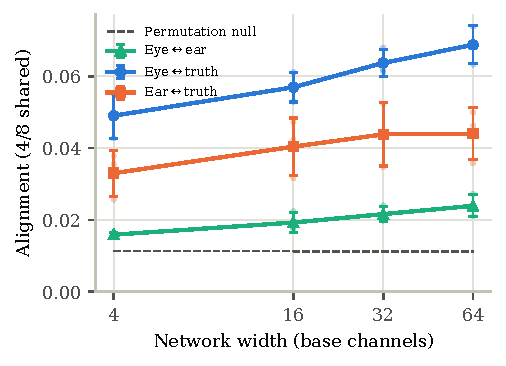
\includegraphics[width=0.55\linewidth]{figures/fig_synth_width.pdf}
  \caption{Width sweep at half overlap ($S=4$, \texttt{contrast\_drift}, $\sigma=0.05$), mean $\pm$ SD over three seeds; faint dots are individual seeds. The dashed line is the eye\lr{}ear permutation null.}
  \label{fig:width}
\end{figure}

\subsection{How much drift, and how much training?}
\label{sec:drift}

The rule comparison left two questions: how convergence depends on the size of the drift, and whether longer training closes the gap to the reference levels. We ran a follow-up at $S=8$, $w=32$, three seeds, with drift $\sigma\in\{0.01,0.02,0.1,0.2,0.4\}$ for 8{,}000 steps (reusing $\sigma=0$, i.e.\ \texttt{contrast\_fresh}, and $\sigma=0.05$ from the runs above), and with $\sigma=0.05$ for 24{,}000 steps. This follow-up was designed after the main results; its predictions were written into the script before it was run: (i) an inverted U in $\sigma$, since small drift approaches the no-drift case and large drift makes the two glimpses nearly unrelated objects; (ii) the ear depends more on drift than the eye; (iii) longer training closes some, but not most, of the gap.

\begin{figure}[t]
  \centering
  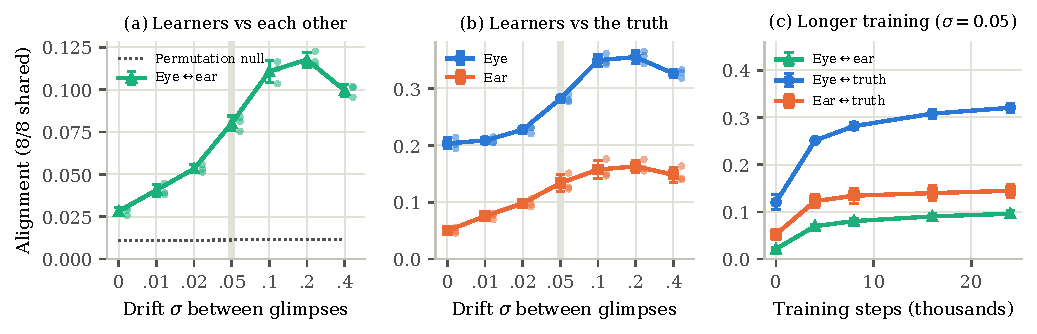
\includegraphics[width=\linewidth]{figures/fig_drift.pdf}
  \caption{Drift sweep and training length ($S=8$, $w=32$, mean $\pm$ SD over three seeds; faint dots are individual seeds). (a, b) Final alignment after 8{,}000 steps as a function of the drift $\sigma$ between glimpses; $\sigma=0$ is \texttt{contrast\_fresh}, and the gray band marks $\sigma=0.05$, the value used in the main experiments. (c) Training for 24{,}000 steps at $\sigma=0.05$.}
  \label{fig:drift}
\end{figure}

\paragraph{An intermediate drift is best.} Alignment rises steadily from $\sigma=0$ and peaks at $\sigma=0.1$--$0.2$ in every seed, then falls at $\sigma=0.4$ in every seed (Figure~\ref{fig:drift}a,b). At $\sigma=0.2$, eye\lr{}ear alignment is $0.118\pm0.004$ (calibrated $0.108\pm0.005$), about 47\% higher than at the value used in the main experiments ($0.080$ at $\sigma=0.05$). The same shape holds for both learners' alignment with the truth. The contrastive loss rises monotonically with $\sigma$ (the task gets harder), so lower training loss does not indicate better recovery of the latent geometry. Prediction (i) is supported. An inverted U is not new in itself: \citet{tian2020views} found a sweet spot in how much information two contrastive views share, measured by downstream accuracy. Here the same shape appears in cross-model convergence and in recovery of the ground-truth latent structure. The main experiments therefore used a suboptimal drift; their qualitative conclusions are unaffected, but their absolute alignments understate what this rule can reach.

\paragraph{The ear depends more on drift.} From $\sigma=0$ to the peak, the ear's alignment with the truth rises by a factor of 3.3 ($0.050\to0.163$) and the eye's by 1.75 ($0.203\to0.355$). The smallest drift already helps the ear substantially ($+51\%$ at $\sigma=0.01$) while barely changing the eye ($+2.5\%$). In absolute terms the two gains are similar ($+0.11$ and $+0.15$), so prediction (ii) holds for relative, not absolute, dependence.

\paragraph{Longer training helps little.} Tripling training at $\sigma=0.05$ raises calibrated eye\lr{}ear alignment from $0.070$ to $0.086$, with diminishing increments ($+0.010$ from 8{,}000 to 16{,}000 steps, $+0.006$ from 16{,}000 to 24{,}000), and the truth alignments from $0.282$ to $0.320$ (eye) and $0.134$ to $0.145$ (ear) (Figure~\ref{fig:drift}c). This closes under two percentage points of the gap between the null and the reference level, as prediction (iii) anticipated. Choosing a better drift did more than tripling training: $\sigma=0.2$ at 8{,}000 steps exceeds $\sigma=0.05$ at 24{,}000 steps ($0.118$ versus $0.096$).

\subsection{Can the correspondence be recovered without pairs?}
\label{sec:unpaired}

If independently trained representations share neighborhood structure, it may be possible to recover which image goes with which sound without any paired data, the premise of unpaired translation between embedding spaces \citep{jha2025vec2vec}. We tested this for every drift value of Section~\ref{sec:drift} ($S=8$, $w=32$, three seeds, retrained). Each learner's final 32-dimensional embeddings of the 1{,}024 test objects were given, with the pairing discarded, to entropic Gromov--Wasserstein optimal transport \citep{peyre2016gromov}, which aligns two point clouds using only their internal distances (cosine distance, normalized by its mean). Three solver settings were run (entropic regularization $0.005$, $0.02$, and an annealed schedule from $0.1$ to $0.005$), and the one with the lowest Gromov--Wasserstein cost was kept, a choice that never uses the true pairing; each Sinkhorn step was solved in the log domain, and numerically degenerate couplings were rejected. The embedding layer was fixed in advance rather than chosen by paired alignment. We report top-1, top-10, and top-50 retrieval of the true partner from the coupling (chance $0.001$, $0.010$, $0.049$) and a \emph{match quality}, one minus the mean true-latent distance between each object and its match divided by the mean distance between random objects (0 for random matching, 1 for perfect). The predictions, recorded before running, were (1) matching follows the inverted U in drift; (2) untrained networks and $\sigma=0$ match at chance; and (3) a null result is possible, because the matcher needs nearly faithful geometry.

\begin{table}[t]
  \centering
  \small
  \caption{Unpaired matching of eye and ear embeddings ($S=8$, $w=32$, 8{,}000 steps; mean $\pm$ SD over three seeds). Paired $M$ is the ordinary (paired) eye\lr{}ear alignment of the same networks, maximized over layers (matching used the embedding layer only); which were retrained for this test and match Section~\ref{sec:drift} to within 0.001. Chance: top-10 0.010, top-50 0.049, quality 0.}
  \label{tab:unpaired}
  \begin{tabular}{lcccc}
    \toprule
    Networks & Paired $M$ & Top-10 & Top-50 & Match quality \\
    \midrule
    Untrained         & $0.022\pm0.003$ & $0.010\pm0.006$ & $0.052\pm0.005$ & $\phantom{-}0.004\pm0.005$ \\
    $\sigma=0$        & $0.028\pm0.002$ & $0.009\pm0.002$ & $0.042\pm0.003$ & $\phantom{-}0.004\pm0.006$ \\
    $\sigma=0.01$     & $0.041\pm0.003$ & $0.010\pm0.002$ & $0.047\pm0.001$ & $\phantom{-}0.001\pm0.002$ \\
    $\sigma=0.02$     & $0.053\pm0.003$ & $0.005\pm0.001$ & $0.036\pm0.005$ & $-0.004\pm0.002$ \\
    $\sigma=0.05$     & $0.080\pm0.005$ & $0.007\pm0.004$ & $0.044\pm0.009$ & $-0.006\pm0.013$ \\
    $\sigma=0.1$      & $0.111\pm0.006$ & $0.010\pm0.003$ & $0.048\pm0.013$ & $-0.001\pm0.022$ \\
    $\sigma=0.2$      & $0.119\pm0.005$ & $0.007\pm0.002$ & $0.038\pm0.014$ & $-0.024\pm0.031$ \\
    $\sigma=0.4$      & $0.100\pm0.004$ & $0.007\pm0.005$ & $0.050\pm0.036$ & $-0.002\pm0.054$ \\
    \bottomrule
  \end{tabular}
\end{table}

\paragraph{The correspondence is not recovered.} Unpaired matching stays at chance for every drift value and seed (Table~\ref{tab:unpaired}): top-1 retrieval never exceeds $0.002$, and match quality averages $-0.005\pm0.023$ over the 21 trained configurations. The largest single value, top-50 retrieval of $0.090$ at $\sigma=0.4$ (seed 0), is not replicated in the other two seeds ($0.040$, $0.021$). The paired alignment of the same networks reproduces the drift sweep, so the networks trained as before; the matcher cannot use their shared structure. Prediction (2) is supported and prediction (1) is not; the null result anticipated as possible in (3) occurred.

\paragraph{How much agreement unpaired matching needs.} To locate the gap, we ran the same matcher on the true latent vectors against noisy copies of themselves ($N=400$ objects, all properties shared), where paired alignment can be dialed directly (Table~\ref{tab:calib}). Recovery is essentially complete when paired alignment is about $0.5$ or more, still mostly successful at $0.45$, and falls away below about $0.3$. The best learners reach a paired alignment of $0.12$ (at $N=1024$; paired alignment decreases with $N$, Table~\ref{tab:scale}, so the comparison is approximate). Neighborhood agreement of the size produced here is thus far below what this method needs: statistically unmistakable convergence (every configuration beats all 20 permutations) is not the same as geometry faithful enough to recover correspondences. The two measures ask different things of the geometry. Mutual $k$-NN rewards any above-chance overlap in each object's ten nearest neighbors; at a paired score of $0.12$, about nine of those ten still differ between the two spaces. Gromov--Wasserstein matching needs the two sets of pairwise distances to agree closely across all objects, close to an isometry, so that each object's position relative to every other identifies it. Local agreement this partial leaves many near-equivalent matchings, and the solver has no basis to prefer the true one. This is a limit of the present learners and of one matching method, not a general impossibility; better learners, other matchers, or a few paired anchors may change it.

\begin{table}[t]
  \centering
  \small
  \caption{Matcher calibration: true latents matched against noisy copies of themselves ($N=400$, $S=8$). Paired alignment of the two point sets versus unpaired match quality and top-1 retrieval.}
  \label{tab:calib}
  \begin{tabular}{cccc}
    \toprule
    Noise SD & Paired $M$ & Match quality & Top-1 \\
    \midrule
    0.05 & 0.73 & 1.00 & 1.00 \\
    0.08 & 0.60 & 0.99 & 0.98 \\
    0.10 & 0.53 & 0.98 & 0.95 \\
    0.12 & 0.45 & 0.89 & 0.80 \\
    0.15 & 0.36 & 0.42 & 0.22 \\
    0.20 & 0.26 & 0.15 & 0.02 \\
    \bottomrule
  \end{tabular}
\end{table}

\subsection{Does alignment fall with evaluation size?}
\label{sec:scale}

The main synthetic evaluation, like the text--vision check, uses 1{,}024 test objects. \citet{koepke2026cave} report that cross-modal alignment falls as evaluation sets grow while coarse agreement holds, and Section~\ref{sec:disc} shows that partially shared perception produces this pattern even for perfect learners (Table~\ref{tab:scale}). To test whether trained learners show it, we trained the eye and ear at $S\in\{8,6,4\}$ (\texttt{contrast\_drift}, $\sigma=0.05$, $w=32$, three seeds) and evaluated each pair on $N\in\{256,1024,4096,8192\}$ new objects, with fine neighborhoods ($k=10$) and coarse ones ($k=N/100$), using a 10-permutation null. $S=8$ is the control: with nothing private, any fall with $N$ must come from learning error. The predictions, recorded before running, were (1) with $k=10$, alignment falls with $N$ at every $S$, including $S=8$; (2) with $k=N/100$, it is roughly constant; (3) for $S<8$, the learned curve falls roughly in proportion to the perfect-learner curve.

\begin{figure}[t]
  \centering
  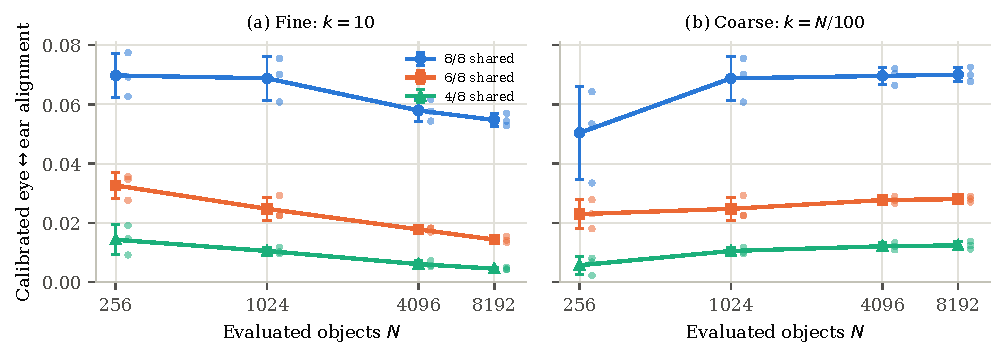
\includegraphics[width=\linewidth]{figures/fig_scale.pdf}
  \caption{Calibrated eye\lr{}ear alignment of trained learners as the number of evaluated objects grows ($\sigma=0.05$, $w=32$, mean $\pm$ SD over three seeds; faint dots are individual seeds). (a) Fine neighborhoods, $k=10$. (b) Coarse neighborhoods, a fixed 1\% of the data. With $N=256$, $k=N/100$ is only 3, and estimates are noisy.}
  \label{fig:scale}
\end{figure}

\paragraph{Fine agreement falls; coarse agreement holds.} With $k=10$, calibrated alignment falls from $N=256$ to $N=8192$ at every overlap level: by 22\% at $S=8$ ($0.070\to0.055$), 56\% at $S=6$ ($0.033\to0.014$), and 68\% at $S=4$ ($0.014\to0.005$) (Figure~\ref{fig:scale}a). From $N=1024$ upward the decline is monotone in every seed except one flat step at $S=8$. With $k=N/100$, alignment is essentially constant from $N=1024$ upward ($0.069$, $0.070$, $0.070$ at $S=8$; $0.025$, $0.028$, $0.028$ at $S=6$; $0.011$, $0.012$, $0.012$ at $S=4$; Figure~\ref{fig:scale}b); at $N=256$ the three-neighbor estimate is lower and noisy. Predictions (1) and (2) are supported: trained learners show the pattern \citet{koepke2026cave} describe, and the control shows that learning error alone produces part of the fine-grained decline, while private properties roughly triple it.

\paragraph{Relative to perfect learners.} At $S=6$, the learners stay at a constant fraction of the perfect-learner level across $N$ (calibrated score divided by the perfect learners' calibrated score: $0.10$ at every $N$), falling in step with it as prediction (3) anticipated. At $S=4$, they fall less steeply than perfect learners, the fraction rising from $0.10$ to $0.17$, so prediction (3) holds at $S=6$ but not at $S=4$. One possible reason, which is speculation, is that the learners encode their private properties only weakly, so those properties reshuffle their neighborhoods less than they reshuffle the latent vectors themselves.

%======================================================================
\section{A sanity check with language and vision models}
\label{sec:textvision}

\paragraph{Setup.} We repeat the measurement of \citet{huh2024platonic} at small scale, on the 1{,}024 image--caption pairs from WIT \citep{srinivasan2021wit} that they released. Captions are embedded with six Pythia models \citep{biderman2023pythia} (70M--2.8B) by mean-pooling each layer's hidden states over non-padding tokens (maximum 256 tokens); images with DINOv2-S, -B, and -L \citep{oquab2023dinov2} using each layer's CLS token. Parameter counts exclude the output head. A randomly initialized Pythia-410M serves as an untrained control. All runs used one NVIDIA RTX 4070 Ti (12\,GB).

\paragraph{Scope.} This check reproduces the original evaluation regime---about a thousand items, one caption per image---which \citet{koepke2026cave} show overstates convergence relative to larger, many-to-many evaluations. It shares human data between the two sides by construction. We include it to confirm that our pipeline reproduces the reported trend and to show the effect of calibration, not as evidence about convergence at scale or about its cause.

\begin{table}[t]
  \centering
  \small
  \caption{Text--vision check. Raw layer-maximized alignment $M$ ($\pm$ SD over 80\% item subsets), the mean of its 20-permutation null $\mu_0$, and the calibrated score $\tilde M$. Every trained and untrained cell exceeded all 20 permutations ($p=0.048$, the minimum attainable).}
  \label{tab:pythia}
  \footnotesize
  \setlength{\tabcolsep}{4pt}
  \begin{tabular}{lr ccc ccc}
    \toprule
    & & \multicolumn{3}{c}{Raw $M$} & \multicolumn{3}{c}{Calibrated $\tilde M$} \\
    \cmidrule(lr){3-5}\cmidrule(lr){6-8}
    Text model & Params (M) & DINOv2-S & DINOv2-B & DINOv2-L & S & B & L \\
    \midrule
    Pythia-410M, random init & 354 & $0.034 \pm 0.002$ & $0.033 \pm 0.002$ & $0.035 \pm 0.002$ & 0.022 & 0.021 & 0.022 \\
    \midrule
    Pythia-70M   & 45   & $0.051 \pm 0.002$ & $0.051 \pm 0.002$ & $0.050 \pm 0.002$ & 0.039 & 0.039 & 0.038 \\
    Pythia-160M  & 124  & $0.056 \pm 0.002$ & $0.057 \pm 0.002$ & $0.058 \pm 0.003$ & 0.045 & 0.045 & 0.046 \\
    Pythia-410M  & 354  & $0.064 \pm 0.002$ & $0.066 \pm 0.003$ & $0.071 \pm 0.002$ & 0.052 & 0.054 & 0.058 \\
    Pythia-1B    & 909  & $0.074 \pm 0.003$ & $0.075 \pm 0.003$ & $0.079 \pm 0.002$ & 0.062 & 0.064 & 0.067 \\
    Pythia-1.4B  & 1312 & $0.073 \pm 0.002$ & $0.076 \pm 0.002$ & $0.077 \pm 0.002$ & 0.062 & 0.064 & 0.065 \\
    Pythia-2.8B  & 2646 & $0.086 \pm 0.003$ & $0.086 \pm 0.003$ & $0.091 \pm 0.002$ & 0.074 & 0.074 & 0.079 \\
    \bottomrule
  \end{tabular}
\end{table}

\paragraph{Results.} Table~\ref{tab:pythia} summarizes the check.
\begin{itemize}
  \item \emph{The null is small and grows only slightly with depth.} The permutation null ranges from 0.0122 to 0.0130 across cells. It correlates with the number of layer pairs searched ($r=0.84$; from 91 pairs for Pythia-70M $\times$ DINOv2-S to 825 for Pythia-2.8B $\times$ DINOv2-L), confirming the depth confound of \citet{groger2026aristotelian}, but for mutual $k$-NN at this scale it amounts to less than 0.001.
  \item \emph{The size trend survives calibration.} Calibrated alignment rises from 0.038--0.039 (Pythia-70M) to 0.074--0.079 (Pythia-2.8B). Least-squares slopes on $\log_2$(parameters) are 0.0057, 0.0059, and 0.0068 per doubling for DINOv2-S, -B, and -L (Pearson $r=0.98$, $0.99$, $0.99$ over six models). Pythia-1.4B does not clearly exceed Pythia-1B (the differences are within one SD), and the next step, to 2.8B, is clearly positive.
  \item \emph{Learning, not architecture, drives most of the effect.} The randomly initialized Pythia-410M reaches a calibrated score of 0.021--0.022, well above the null, and in every case its best layer is the token-embedding layer. This is consistent with lexical overlap: even random embeddings preserve which tokens a caption contains, and captions sharing words tend to describe similar images. The trained Pythia-410M scores 0.052--0.058, about 2.5 times the untrained level.
\end{itemize}
Within the limits stated above, this reproduces the trend reported by \citet{huh2024platonic} and shows that it is not an artifact of the layer search. It says nothing about whether the trend persists at larger evaluation scales, where \citet{koepke2026cave} find that it does not, or about whether it reflects shared data.


%======================================================================
\section{Discussion}
\label{sec:disc}

\paragraph{What the evidence supports.} In the synthetic world, two learners that never share data converge in proportion to the fraction of the world they perceive in common, not at all when they share nothing, and, from half overlap upward, each moves toward the world's true latent structure while doing so. Within this setting that is what (H) claims, and the shared-data explanation is excluded by construction. It is also what identifiability theory predicts \citep{zimmermann2021contrastive,vonkugelgen2021self,daunhawer2023identifiability}; the experiment confirms that the prediction holds for finite networks on rendered images and sounds with disjoint training data, and that reconstruction and contrastive learning without drift fall well short. Convergence was strongest when positive pairs were neither too close nor too far apart in latent space. A more accurate statement of (H) for our data is therefore that learners whose objective recovers the latent geometry converge on the part of the world they share.

\paragraph{Relation to other evidence.} \citet{tjandrasuwita2025emergence} find that alignment grows with capacity only when modalities are highly redundant; we see a small but consistent capacity effect at half overlap, in a setting that differs in objective, data, input, and metric. Our low absolute alignments at partial overlap are consistent with their emphasis on redundancy: private properties limit neighborhood agreement even for perfect learners (the ``Perfect'' column of Table~\ref{tab:synth}). The text--vision check cannot separate shared data from a shared world. Our synthetic results show that a shared world \emph{can} produce convergence without shared data, not how much of the convergence between web-trained models it explains; real models trained on disjoint real-world data, evaluated at scale, would be a natural bridge.

\paragraph{A candidate mechanism for the scale effect.} \citet{koepke2026cave} report that language--vision alignment falls roughly sixteenfold as the evaluation set grows from about a thousand to millions of items, and that models agree on coarse categories but not on which instances are most similar; they interpret this through von Uexküll's notion of an \emph{umwelt}, each model building its own structure from its modality and data. Our overlap manipulation is a minimal model of partially shared umwelten, and its reference levels suggest a mechanism. Table~\ref{tab:scale} gives the alignment of \emph{perfect} learners---features equal to their own latent vectors, with no learning error---as the number of evaluated objects $N$ grows. With a fixed $k=10$, agreement falls with $N$ whenever each sense has any private property (from 0.55 to 0.34 with one private property of eight), and not at all when everything is shared. When neighborhoods are instead a fixed fraction of the data ($k=N/100$), agreement is essentially constant across $N$. The decline is therefore a matter of resolution: as sampling becomes denser, each object's nearest neighbors are decided by finer differences, and private properties, invisible to the other learner, make up a growing share of them. Coarse agreement survives while fine agreement erodes, which is the pattern \citet{koepke2026cave} describe. Partially shared perception can thus produce both of their observations even for learners that recover the shared structure exactly. Trained learners show the same qualitative pattern, with learning error contributing a smaller share of the decline, but the mechanism is only partly confirmed for them: their decline tracks the perfect learners' in proportion at $S=6$ and is shallower at $S=4$, for reasons we did not test (Section~\ref{sec:scale}). This does not show that it is the cause in their models, where imperfect learning and differences in data may also contribute, but it suggests that falling fine-grained alignment at scale is compatible with convergence on shared structure, and that the umwelt and Platonic accounts may describe different resolutions of the same situation.

\begin{table}[t]
  \centering
  \small
  \caption{Perfect-learner alignment $M(Z^e,Z^a)$ versus the number of evaluated objects $N$, for $S$ of 8 properties shared (means over three draws; SD $\leq 0.03$ throughout). Left: fixed $k=10$. Right: $k=N/100$, a fixed fraction of the data (chance is $k/(N-1)$: from $0.039$ to $0.001$ for $k=10$, and about $0.01$ for $k=N/100$).}
  \label{tab:scale}
  \begin{tabular}{r cccc c cccc}
    \toprule
    & \multicolumn{4}{c}{$k=10$} && \multicolumn{4}{c}{$k=N/100$} \\
    \cmidrule(lr){2-5}\cmidrule(lr){7-10}
    $N$ & $S=8$ & $S=7$ & $S=6$ & $S=4$ && $S=8$ & $S=7$ & $S=6$ & $S=4$ \\
    \midrule
    256  & 1.000 & 0.551 & 0.367 & 0.175 && 1.000 & 0.442 & 0.238 & 0.094 \\
    1024 & 1.000 & 0.449 & 0.259 & 0.082 && 1.000 & 0.449 & 0.259 & 0.082 \\
    4096 & 1.000 & 0.374 & 0.175 & 0.041 && 1.000 & 0.468 & 0.261 & 0.087 \\
    8192 & 1.000 & 0.338 & 0.144 & 0.028 && 1.000 & 0.467 & 0.261 & 0.088 \\
    \bottomrule
  \end{tabular}
\end{table}

\paragraph{Implications and open hypotheses.} First, \emph{unpaired alignment}: we hypothesized that training choices such as the drift between views (in practice, augmentation strength or the time gap between video frames) might determine how translatable independently trained models are. Drift changed paired alignment by a factor of four, yet unpaired matching stayed at chance, because even the best learners fall far short of the agreement the matcher requires (Section~\ref{sec:unpaired}). Second, \emph{timescale}: in natural learners, the analogue of drift is how much the world changes between successive moments of perception, the intuition behind slow feature analysis \citep{wiskott2002slow}; in machine learning, it is the gap between frames of a video or the strength of augmentation. Two learners that sample a shared world on very different timescales may converge less than their shared perception alone would allow; training the eye and ear with different $\sigma$ would test this. Third, \emph{evaluation design}: the exploratory four-glimpse evaluation (Appendix~\ref{app:dev}) raised alignment from below $0.06$ to about $0.30$, because several glimpses of one object are trivially each other's neighbors in both spaces. Many-to-many benchmarks, with several captions per image or several views per object, can inflate or deflate alignment depending on how such near-duplicates are counted, so evaluation choices of this kind need to be reported with the score. Fourth, \emph{other species}: because even perfect learners agree little on neighborhoods when many properties are private, low alignment between, say, a model of human language and a model of animal vocalizations would not by itself show that no structure is shared.

%======================================================================
\section{Limitations}

\begin{itemize}
  \item \textbf{Scale.} The synthetic world has 8 latent dimensions per sense and networks with under one million parameters. The text--vision check uses at most 2.8B parameters and 1{,}024 items, a regime known to overstate cross-modal convergence \citep{koepke2026cave}.
  \item \textbf{Evaluation regime.} Most synthetic results use 1{,}024 objects with exactly one image and one sound each, the regime \citet{koepke2026cave} show inflates cross-modal alignment for web data. Section~\ref{sec:scale} shows how the trained learners' alignment changes with $N$: comparisons across conditions at fixed $N$ are unaffected, but absolute fine-grained alignments, including the comparison with the matcher's calibration threshold (Section~\ref{sec:unpaired}), would be lower on larger evaluation sets. In the synthetic world the one-to-one correspondence is real by construction; we did not replicate the many-to-many captioning setting of \citet{koepke2026cave}.
  \item \textbf{Seeds.} Three seeds per synthetic configuration resolve the large effects (overlap, learning rule) but leave small differences, such as between adjacent widths, uncertain.
  \item \textbf{Toy world.} Latents are independent and uniform, renderers are fixed random networks, and nuisance is simple. Real worlds have hierarchical, correlated, and causal structure.
  \item \textbf{Rule selection and follow-up.} The four rules were fixed before the runs reported here, but after development runs that shaped them (Appendix~\ref{app:dev}). They are illustrative contrasts, not a survey of learning rules. The drift sweep was designed after the main results, with its predictions recorded before it ran.
  \item \textbf{Hyperparameters.} The main experiments used $\sigma=0.05$, which the drift sweep shows is below the best value; the sweep itself covers only full overlap and one width. Temperature, batch size, learning rate, and architecture were not tuned.
  \item \textbf{Metric.} We use one local neighborhood metric, cosine mutual $k$-NN with $k=10$ (and $k=N/100$ in Section~\ref{sec:scale}), and a simplified permutation calibration. Truth alignment applies cosine similarity to uncentered latents (Section~\ref{sec:formal}). Global metrics and metric geometry may behave differently \citep{groger2026aristotelian,you2026structure}. The unpaired test uses one matching method, Gromov--Wasserstein transport, and its calibration used fewer objects than the main evaluation.
  \item \textbf{Cause in real data.} The synthetic results bear on whether a shared world \emph{can} produce convergence without shared data; they do not establish how much of the convergence observed between web-trained models it explains.
\end{itemize}

%======================================================================
\section{Conclusion}

This confirmatory study checked a prediction of identifiability theory in a regime the theory does not directly cover. In a synthetic world with two senses, separately trained learners that shared no data converged in proportion to how much of the world they perceived in common, and, from half overlap upward, each approached the world's true latent structure. The effect was strong only when contrastive glimpses came from an object that changed between them, which approximates the condition the theory requires, and peaked at an intermediate drift. The results support the view that representational convergence can arise from learning about a shared world rather than from sharing data. Two findings temper it: the convergence was statistically clear but far too weak for unpaired matching, and with partially shared perception fine-grained agreement falls as evaluation sets grow while coarse agreement holds, a candidate reconciliation of recent evidence against convergence at scale with convergence on shared structure. Going beyond confirmation requires conditions where the theory makes no guarantee: correlated or hierarchical latents, occlusion, and real models trained on disjoint data.

\section*{Reproducibility}
{\sloppy All code and raw results are included in the accompanying archive (\href{https://doi.org/10.5281/zenodo.23445191}{doi:10.5281/zenodo.23445191}) and at \url{https://github.com/jbussin/senses-converge}, with a README; an interactive summary is at \url{https://jbussin.github.io/senses-converge/}. \texttt{synthetic\_world.py} defines the world, learners, and metric; \texttt{synthetic\_robustness.py} produced the overlap, learning-rule, and width experiments; \texttt{drift\_sweep.py} produced the drift sweep and longer-training runs (Section~\ref{sec:drift}); \texttt{unpaired\_alignment.py} produced the unpaired matching results and, with the \texttt{-{}-calibrate} option, the matcher calibration (Section~\ref{sec:unpaired}; it requires the POT library); \texttt{scale\_eval.py} produced the evaluation-size results (Section~\ref{sec:scale}); \texttt{perfect\_learner\_scale.py} computes Table~\ref{tab:scale}; \texttt{platonic\_test.py} produced the text--vision check; and \texttt{make\_figures\_v2.py} regenerates Figures~1--4 and the numbers in Table~\ref{tab:synth} and Sections~\ref{sec:drift} and~\ref{sec:scale} from the included result files; Tables~\ref{tab:unpaired}--\ref{tab:pythia} are read directly from the result files of the scripts named above. All experiments ran on one NVIDIA RTX 4070 Ti (12\,GB); a synthetic configuration takes about two minutes per 8{,}000 steps. Software: Python 3.14, PyTorch 2.11 (CUDA 12.8), Transformers 5.17.\par}

\section*{Acknowledgments}
Experiment code, analysis, and drafting were done with the assistance of Claude, an AI system developed by Anthropic. The author ran all experiments and is responsible for the content.

\bibliographystyle{plainnat}
\bibliography{refs}

\appendix
\section{Renderer details}
\label{app:render}

In Eq.~\eqref{eq:render}, the feature maps satisfy $\phi_e:[0,1]^8\to(0,1)^{36}$ and $\phi_a:[0,1]^8\to(0,1)^{18}$. The eye renderer places six blobs with centers $\mu_j=0.15+0.7(u_j,v_j)+\delta$, widths $r_j=0.04+0.16\rho_j$, and colors $c_j\in(0,1)^3$ read from $\phi_e$. With $\tilde x_k(q)=\sum_j c_{jk}\exp\!\big(-\lVert q-\mu_j\rVert^2/2r_j^2\big)$ for color channel $k$ and pixel position $q\in[0,1]^2$,
\begin{equation}
  x^{e}_k(q)=\beta\,\frac{\tilde x_k(q)}{\max_{q',k'}\tilde x_{k'}(q')}+\epsilon ,
\end{equation}
with nuisance $\nu^{e}=(\delta,\beta,\epsilon)$: $\delta\sim\mathcal U([-0.12,0.12]^2)$, $\beta\sim\mathcal U[0.7,1.3]$, $\epsilon\sim\mathcal N(0,0.05^2)$ per pixel and channel. The ear renderer sums six tones with frequencies $f_j=5+115\,\phi_{a,j1}$ (cycles per clip), amplitudes $a_j=\phi_{a,j2}$, and decay rates $\lambda_j=6\,\phi_{a,j3}$. With $\tilde x(t)=\sum_j a_j\,\mathbf 1[t\ge t_0]\,e^{-\lambda_j(t-t_0)}\sin\!\big(2\pi f_j(t-t_0)+\theta_j\big)$ for $t\in[0,1]$,
\begin{equation}
  x^{a}(t)=\alpha\,\frac{\tilde x(t)}{\max_{t'}\lvert\tilde x(t')\rvert}+\epsilon,
\end{equation}
with nuisance $\nu^{a}=(t_0,\theta,\alpha,\epsilon)$: $t_0\sim\mathcal U[0,0.15]$, $\theta_j\sim\mathcal U[0,2\pi)$, $\alpha\sim\mathcal U[0.7,1.3]$, $\epsilon\sim\mathcal N(0,0.05^2)$ per sample. The ear's fixed front end $C$ uses a Hann window of 128 samples with hop 32, cropped to the lowest 64 frequency bins and first 32 frames, and the reconstruction rule's decoder mirrors the encoder.

\section{Development runs and an exploratory evaluation}
\label{app:dev}

While developing the experiment on a CPU, we tried the configurations in Table~\ref{tab:explore} at $S=8$, $w=16$, one seed, and short budgets. Reconstruction did not change eye\lr{}ear alignment; contrastive learning on a fixed set of objects converged weakly with or without the cochlear front end; adding fresh objects and drift produced clear convergence. The robustness runs later showed that drift, not fresh objects, was the decisive ingredient. These runs motivated the four pre-specified rules of Section~\ref{sec:synthetic}. The reconstruction row used an earlier version of the world without per-glimpse viewing nuisance and with a raw-waveform ear.

\begin{table}[h]
  \centering
  \small
  \caption{Development runs ($S=8$, $w=16$, CPU, one seed). Budgets differ across rows. Arrows give untrained $\to$ trained where both were recorded.}
  \label{tab:explore}
  \begin{tabular}{lcccc}
    \toprule
    Configuration & Steps & Eye\lr{}ear & Eye\lr{}truth & Ear\lr{}truth \\
    \midrule
    Denoising reconstruction, raw audio, fixed set & 600 & $0.020 \to 0.021$ & $0.187$ & $0.039$ \\
    Contrastive, raw audio, fixed set & 2400 & $0.014 \to 0.025$ & $0.107 \to 0.152$ & $0.016 \to 0.048$ \\
    Contrastive, cochlea, fixed set & 1200 & $0.023 \to 0.025$ & $0.107 \to 0.146$ & $0.056 \to 0.053$ \\
    Contrastive, cochlea, fresh objects + drift & 1200 & $0.023 \to 0.052$ & $0.107 \to 0.206$ & $0.056 \to 0.098$ \\
    \bottomrule
  \end{tabular}
\end{table}

\paragraph{Exploratory multi-glimpse evaluation.} The evaluation-size runs (Section~\ref{sec:scale}) also evaluated each trained pair on 1{,}024 objects with four independent glimpses per sense, with no prediction recorded. Calibrated alignment with $k=10$ rose to about $0.30$ at every $S$, because glimpses of the same object neighbor each other in both spaces and so count as shared neighbors. This measures invariance to nuisance, not the many-to-many captioning setting of \citet{koepke2026cave}, and we do not interpret it further.

\end{document}
